\documentclass[]{article}
\usepackage{lmodern}
\usepackage{amssymb,amsmath}
\usepackage{ifxetex,ifluatex}
\usepackage{fixltx2e} % provides \textsubscript
\ifnum 0\ifxetex 1\fi\ifluatex 1\fi=0 % if pdftex
  \usepackage[T1]{fontenc}
  \usepackage[utf8]{inputenc}
\else % if luatex or xelatex
  \ifxetex
    \usepackage{mathspec}
  \else
    \usepackage{fontspec}
  \fi
  \defaultfontfeatures{Ligatures=TeX,Scale=MatchLowercase}
\fi
% use upquote if available, for straight quotes in verbatim environments
\IfFileExists{upquote.sty}{\usepackage{upquote}}{}
% use microtype if available
\IfFileExists{microtype.sty}{%
\usepackage{microtype}
\UseMicrotypeSet[protrusion]{basicmath} % disable protrusion for tt fonts
}{}
\usepackage[margin=1in]{geometry}
\usepackage{hyperref}
\hypersetup{unicode=true,
            pdftitle={Reproducible Research - Project 1 - FitBit Data.Rmd},
            pdfborder={0 0 0},
            breaklinks=true}
\urlstyle{same}  % don't use monospace font for urls
\usepackage{color}
\usepackage{fancyvrb}
\newcommand{\VerbBar}{|}
\newcommand{\VERB}{\Verb[commandchars=\\\{\}]}
\DefineVerbatimEnvironment{Highlighting}{Verbatim}{commandchars=\\\{\}}
% Add ',fontsize=\small' for more characters per line
\usepackage{framed}
\definecolor{shadecolor}{RGB}{248,248,248}
\newenvironment{Shaded}{\begin{snugshade}}{\end{snugshade}}
\newcommand{\KeywordTok}[1]{\textcolor[rgb]{0.13,0.29,0.53}{\textbf{#1}}}
\newcommand{\DataTypeTok}[1]{\textcolor[rgb]{0.13,0.29,0.53}{#1}}
\newcommand{\DecValTok}[1]{\textcolor[rgb]{0.00,0.00,0.81}{#1}}
\newcommand{\BaseNTok}[1]{\textcolor[rgb]{0.00,0.00,0.81}{#1}}
\newcommand{\FloatTok}[1]{\textcolor[rgb]{0.00,0.00,0.81}{#1}}
\newcommand{\ConstantTok}[1]{\textcolor[rgb]{0.00,0.00,0.00}{#1}}
\newcommand{\CharTok}[1]{\textcolor[rgb]{0.31,0.60,0.02}{#1}}
\newcommand{\SpecialCharTok}[1]{\textcolor[rgb]{0.00,0.00,0.00}{#1}}
\newcommand{\StringTok}[1]{\textcolor[rgb]{0.31,0.60,0.02}{#1}}
\newcommand{\VerbatimStringTok}[1]{\textcolor[rgb]{0.31,0.60,0.02}{#1}}
\newcommand{\SpecialStringTok}[1]{\textcolor[rgb]{0.31,0.60,0.02}{#1}}
\newcommand{\ImportTok}[1]{#1}
\newcommand{\CommentTok}[1]{\textcolor[rgb]{0.56,0.35,0.01}{\textit{#1}}}
\newcommand{\DocumentationTok}[1]{\textcolor[rgb]{0.56,0.35,0.01}{\textbf{\textit{#1}}}}
\newcommand{\AnnotationTok}[1]{\textcolor[rgb]{0.56,0.35,0.01}{\textbf{\textit{#1}}}}
\newcommand{\CommentVarTok}[1]{\textcolor[rgb]{0.56,0.35,0.01}{\textbf{\textit{#1}}}}
\newcommand{\OtherTok}[1]{\textcolor[rgb]{0.56,0.35,0.01}{#1}}
\newcommand{\FunctionTok}[1]{\textcolor[rgb]{0.00,0.00,0.00}{#1}}
\newcommand{\VariableTok}[1]{\textcolor[rgb]{0.00,0.00,0.00}{#1}}
\newcommand{\ControlFlowTok}[1]{\textcolor[rgb]{0.13,0.29,0.53}{\textbf{#1}}}
\newcommand{\OperatorTok}[1]{\textcolor[rgb]{0.81,0.36,0.00}{\textbf{#1}}}
\newcommand{\BuiltInTok}[1]{#1}
\newcommand{\ExtensionTok}[1]{#1}
\newcommand{\PreprocessorTok}[1]{\textcolor[rgb]{0.56,0.35,0.01}{\textit{#1}}}
\newcommand{\AttributeTok}[1]{\textcolor[rgb]{0.77,0.63,0.00}{#1}}
\newcommand{\RegionMarkerTok}[1]{#1}
\newcommand{\InformationTok}[1]{\textcolor[rgb]{0.56,0.35,0.01}{\textbf{\textit{#1}}}}
\newcommand{\WarningTok}[1]{\textcolor[rgb]{0.56,0.35,0.01}{\textbf{\textit{#1}}}}
\newcommand{\AlertTok}[1]{\textcolor[rgb]{0.94,0.16,0.16}{#1}}
\newcommand{\ErrorTok}[1]{\textcolor[rgb]{0.64,0.00,0.00}{\textbf{#1}}}
\newcommand{\NormalTok}[1]{#1}
\usepackage{graphicx,grffile}
\makeatletter
\def\maxwidth{\ifdim\Gin@nat@width>\linewidth\linewidth\else\Gin@nat@width\fi}
\def\maxheight{\ifdim\Gin@nat@height>\textheight\textheight\else\Gin@nat@height\fi}
\makeatother
% Scale images if necessary, so that they will not overflow the page
% margins by default, and it is still possible to overwrite the defaults
% using explicit options in \includegraphics[width, height, ...]{}
\setkeys{Gin}{width=\maxwidth,height=\maxheight,keepaspectratio}
\IfFileExists{parskip.sty}{%
\usepackage{parskip}
}{% else
\setlength{\parindent}{0pt}
\setlength{\parskip}{6pt plus 2pt minus 1pt}
}
\setlength{\emergencystretch}{3em}  % prevent overfull lines
\providecommand{\tightlist}{%
  \setlength{\itemsep}{0pt}\setlength{\parskip}{0pt}}
\setcounter{secnumdepth}{0}
% Redefines (sub)paragraphs to behave more like sections
\ifx\paragraph\undefined\else
\let\oldparagraph\paragraph
\renewcommand{\paragraph}[1]{\oldparagraph{#1}\mbox{}}
\fi
\ifx\subparagraph\undefined\else
\let\oldsubparagraph\subparagraph
\renewcommand{\subparagraph}[1]{\oldsubparagraph{#1}\mbox{}}
\fi

%%% Use protect on footnotes to avoid problems with footnotes in titles
\let\rmarkdownfootnote\footnote%
\def\footnote{\protect\rmarkdownfootnote}

%%% Change title format to be more compact
\usepackage{titling}

% Create subtitle command for use in maketitle
\newcommand{\subtitle}[1]{
  \posttitle{
    \begin{center}\large#1\end{center}
    }
}

\setlength{\droptitle}{-2em}
  \title{Reproducible Research - Project 1 - FitBit Data.Rmd}
  \pretitle{\vspace{\droptitle}\centering\huge}
  \posttitle{\par}
  \author{}
  \preauthor{}\postauthor{}
  \date{}
  \predate{}\postdate{}


\begin{document}
\maketitle

\subsubsection{About}\label{about}

This was the first project for the \textbf{Reproducible Research} course
in
\href{https://www.coursera.org/learn/reproducible-research/home/welcome}{Coursera's
Data Science specialization} track. The purpose of this project was to
answer a series of questions using data collected from a
\href{http://en.wikipedia.org/wiki/Fitbit}{FitBit}.

\subsection{Synopsis}\label{synopsis}

The purpose of this project was to practice:

\begin{itemize}
\tightlist
\item
  downloading, loading and preprocessing data
\item
  imputing missing values
\item
  interpreting data to answer research questions
\end{itemize}

\subsection{Data}\label{data}

The data for this assignment was downloaded from the course web site:

\begin{itemize}
\tightlist
\item
  Dataset:
  \href{https://d396qusza40orc.cloudfront.net/repdata\%2Fdata\%2Factivity.zip}{Activity
  monitoring data} {[}52K{]}
\end{itemize}

The variables included in this dataset are:

\begin{itemize}
\item
  \textbf{steps}: Number of steps taking in a 5-minute interval (missing
  values are coded as \texttt{NA})
\item
  \textbf{date}: The date on which the measurement was taken in
  YYYY-MM-DD format (YYYY for year, MM for month, DD for day)
\item
  \textbf{interval}: Identifier for the 5-minute interval in which
  measurement was taken
\end{itemize}

The dataset is stored in a comma-separated-value (CSV) file and there
are a total of 17,568 observations in this dataset.

\subsection{downloading, loading and preprocessing the
data}\label{downloading-loading-and-preprocessing-the-data}

Download, unzip and load data into data frame \texttt{data}.

\begin{Shaded}
\begin{Highlighting}[]
\ControlFlowTok{if}\NormalTok{(}\OperatorTok{!}\KeywordTok{file.exists}\NormalTok{(}\StringTok{"getdata-projectfiles-UCI HAR Dataset.zip"}\NormalTok{)) \{}
    \ControlFlowTok{if}\NormalTok{(}\OperatorTok{!}\KeywordTok{dir.exists}\NormalTok{(}\StringTok{'data'}\NormalTok{))\{}\KeywordTok{dir.create}\NormalTok{(}\StringTok{'data'}\NormalTok{)\}}
\NormalTok{    data.zip <-}\StringTok{ 'data/repdata-data-activity.zip'}\NormalTok{;}
    \KeywordTok{download.file}\NormalTok{(}\StringTok{"http://d396qusza40orc.cloudfront.net/repdata%2Fdata%2Factivity.zip"}\NormalTok{,data.zip)}
    \KeywordTok{unzip}\NormalTok{(data.zip, }\DataTypeTok{exdir =} \StringTok{'data'}\NormalTok{)}
    \KeywordTok{unlink}\NormalTok{(data.zip)}
\NormalTok{\}}

\ControlFlowTok{if}\NormalTok{(}\StringTok{"data.table"} \OperatorTok\StringTok{ }\KeywordTok{rownames}\NormalTok{(}\KeywordTok{installed.packages}\NormalTok{()) }\OperatorTok{==}\StringTok{ }\OtherTok{FALSE}\NormalTok{) \{}\KeywordTok{install.packages}\NormalTok{(}\StringTok{"data.table"}\NormalTok{)\}}
\KeywordTok{library}\NormalTok{(data.table);}

\ControlFlowTok{if}\NormalTok{(}\StringTok{"lubridate"} \OperatorTok\StringTok{ }\KeywordTok{rownames}\NormalTok{(}\KeywordTok{installed.packages}\NormalTok{()) }\OperatorTok{==}\StringTok{ }\OtherTok{FALSE}\NormalTok{) \{}\KeywordTok{install.packages}\NormalTok{(}\StringTok{"lubridate"}\NormalTok{)\}}
\KeywordTok{library}\NormalTok{(lubridate)}
\end{Highlighting}
\end{Shaded}

\begin{verbatim}
## 
## Attaching package: 'lubridate'
\end{verbatim}

\begin{verbatim}
## The following objects are masked from 'package:data.table':
## 
##     hour, isoweek, mday, minute, month, quarter, second, wday,
##     week, yday, year
\end{verbatim}

\begin{verbatim}
## The following object is masked from 'package:base':
## 
##     date
\end{verbatim}

\begin{Shaded}
\begin{Highlighting}[]
\NormalTok{data <-}\StringTok{ }\KeywordTok{fread}\NormalTok{(}\StringTok{"data/activity.csv"}\NormalTok{)}
\end{Highlighting}
\end{Shaded}

\subsection{What is mean total number of steps taken per
day?}\label{what-is-mean-total-number-of-steps-taken-per-day}

Sum steps by day, create Histogram, and calculate mean and median.

\begin{Shaded}
\begin{Highlighting}[]
\NormalTok{steps_by_day <-}\StringTok{ }\KeywordTok{aggregate}\NormalTok{(steps }\OperatorTok{~}\StringTok{ }\NormalTok{date, data, sum);}
\KeywordTok{summary}\NormalTok{(steps_by_day);}
\end{Highlighting}
\end{Shaded}

\begin{verbatim}
##      date               steps      
##  Length:53          Min.   :   41  
##  Class :character   1st Qu.: 8841  
##  Mode  :character   Median :10765  
##                     Mean   :10766  
##                     3rd Qu.:13294  
##                     Max.   :21194
\end{verbatim}

\begin{Shaded}
\begin{Highlighting}[]
\KeywordTok{hist}\NormalTok{(steps_by_day}\OperatorTok{$}\NormalTok{steps, }\DataTypeTok{main =} \KeywordTok{paste}\NormalTok{(}\StringTok{"Total Steps Each Day"}\NormalTok{), }\DataTypeTok{col=}\StringTok{"blue"}\NormalTok{, }\DataTypeTok{xlab=}\StringTok{"Number of Steps"}\NormalTok{, }\DataTypeTok{breaks =} \DecValTok{16}\NormalTok{);}
\end{Highlighting}
\end{Shaded}

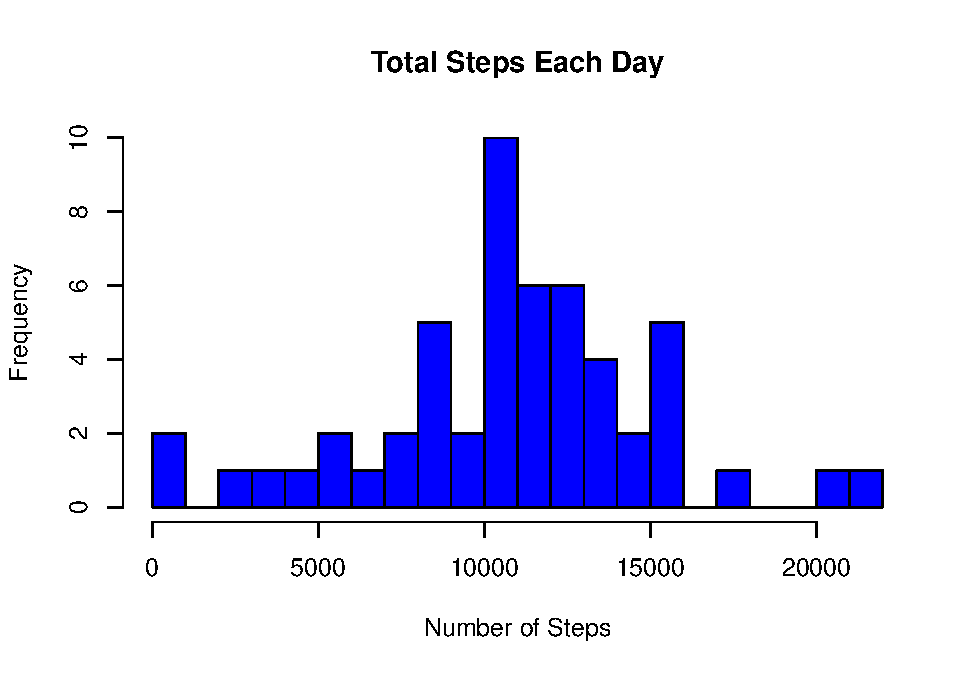
\includegraphics{PA1_template_files/figure-latex/unnamed-chunk-2-1.pdf}

\begin{Shaded}
\begin{Highlighting}[]
\NormalTok{rmean <-}\StringTok{ }\KeywordTok{mean}\NormalTok{(steps_by_day}\OperatorTok{$}\NormalTok{steps);}
\NormalTok{rmedian <-}\StringTok{ }\KeywordTok{median}\NormalTok{(steps_by_day}\OperatorTok{$}\NormalTok{steps);}
\NormalTok{a <-}\StringTok{ }\KeywordTok{sprintf}\NormalTok{(}\StringTok{"The mean is %3.1f and median is %3.1f"}\NormalTok{, rmean, rmedian)}
\end{Highlighting}
\end{Shaded}

The mean is 10766.2 and median is 10765.0

\subsection{What is the average daily activity
pattern?}\label{what-is-the-average-daily-activity-pattern}

\begin{itemize}
\tightlist
\item
  Calculate average steps for each interval for all days.
\item
  Plot the average number steps per day by interval.
\item
  Find interval with most average steps.
\end{itemize}

\begin{Shaded}
\begin{Highlighting}[]
\NormalTok{steps_by_interval <-}\StringTok{ }\KeywordTok{aggregate}\NormalTok{(steps }\OperatorTok{~}\StringTok{ }\NormalTok{interval, data, mean)}

\KeywordTok{plot}\NormalTok{(steps_by_interval}\OperatorTok{$}\NormalTok{interval, steps_by_interval}\OperatorTok{$}\NormalTok{steps, }
     \DataTypeTok{type=}\StringTok{"l"}\NormalTok{, }\DataTypeTok{xlab=}\StringTok{"Interval"}\NormalTok{, }\DataTypeTok{ylab=}\StringTok{"Number of Steps"}\NormalTok{,}
     \DataTypeTok{main=}\StringTok{"Average Number of Steps per Day by Interval"}\NormalTok{)}
\end{Highlighting}
\end{Shaded}

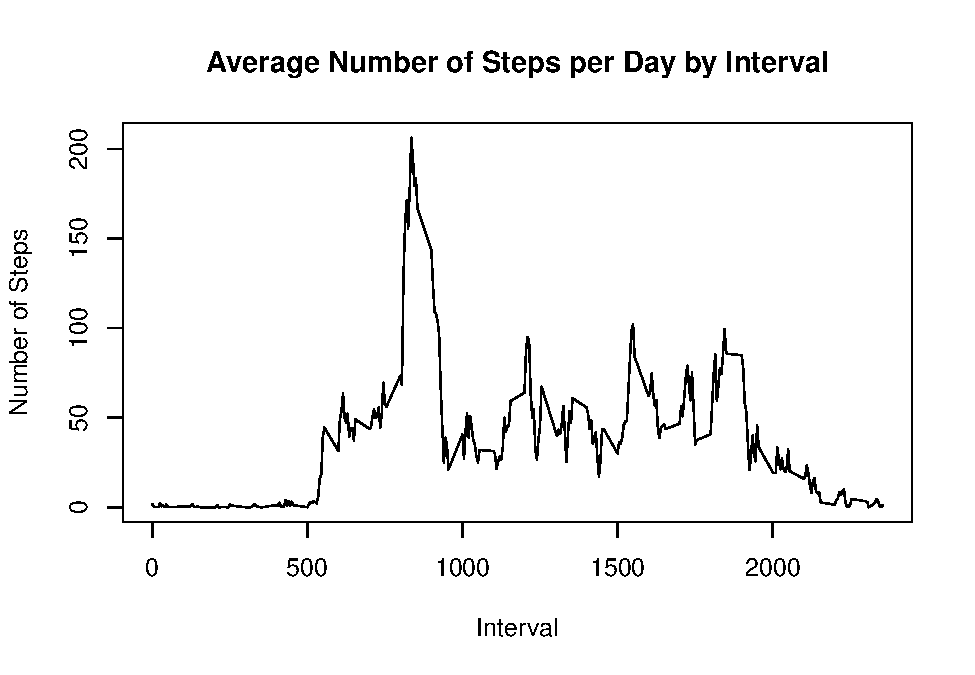
\includegraphics{PA1_template_files/figure-latex/unnamed-chunk-3-1.pdf}

\begin{Shaded}
\begin{Highlighting}[]
\NormalTok{max_interval <-}\StringTok{ }\NormalTok{steps_by_interval[}\KeywordTok{which.max}\NormalTok{(steps_by_interval}\OperatorTok{$}\NormalTok{steps),}\DecValTok{1}\NormalTok{]}
\end{Highlighting}
\end{Shaded}

The 5-minute interval, on average across all the days in the data set,
containing the maximum number of steps is 835.

\subsection{Impute missing values. Compare imputed to non-imputed
data.}\label{impute-missing-values.-compare-imputed-to-non-imputed-data.}

Missing data needed to be imputed. Only a simple imputation approach was
required for this assignment. Missing values were imputed by inserting
the average for each interval. Thus, if interval 10 was missing on
10-02-2012, the average for that interval for all days (0.1320755),
replaced the NA.

\begin{Shaded}
\begin{Highlighting}[]
\NormalTok{q.incomplete <-}\StringTok{ }\KeywordTok{sum}\NormalTok{(}\OperatorTok{!}\KeywordTok{complete.cases}\NormalTok{(data))}
\NormalTok{imputed_data <-}\StringTok{ }\KeywordTok{transform}\NormalTok{(data, }\DataTypeTok{steps =} \KeywordTok{ifelse}\NormalTok{(}\KeywordTok{is.na}\NormalTok{(data}\OperatorTok{$}\NormalTok{steps), steps_by_interval}\OperatorTok{$}\NormalTok{steps[}\KeywordTok{match}\NormalTok{(data}\OperatorTok{$}\NormalTok{interval, steps_by_interval}\OperatorTok{$}\NormalTok{interval)], data}\OperatorTok{$}\NormalTok{steps))}
\end{Highlighting}
\end{Shaded}

Zeroes were imputed for 10-01-2012 because it was the first day and
would have been over 9,000 steps higher than the following day, which
had only 126 steps. NAs then were assumed to be zeros to fit the rising
trend of the data.

\begin{Shaded}
\begin{Highlighting}[]
\NormalTok{imputed_data[}\KeywordTok{as.character}\NormalTok{(imputed_data}\OperatorTok{$}\NormalTok{date) }\OperatorTok{==}\StringTok{ "2012-10-01"}\NormalTok{, }\DecValTok{1}\NormalTok{] <-}\StringTok{ }\DecValTok{0}
\end{Highlighting}
\end{Shaded}

Recount total steps by day and create Histogram.

\begin{Shaded}
\begin{Highlighting}[]
\NormalTok{steps_by_day_i <-}\StringTok{ }\KeywordTok{aggregate}\NormalTok{(steps }\OperatorTok{~}\StringTok{ }\NormalTok{date, imputed_data, sum)}
\KeywordTok{hist}\NormalTok{(steps_by_day_i}\OperatorTok{$}\NormalTok{steps, }\DataTypeTok{main =} \KeywordTok{paste}\NormalTok{(}\StringTok{"Total Steps Each Day"}\NormalTok{), }\DataTypeTok{col=}\StringTok{"blue"}\NormalTok{, }\DataTypeTok{xlab=}\StringTok{"Number of Steps"}\NormalTok{, }\DataTypeTok{breaks =} \DecValTok{16}\NormalTok{)}

\CommentTok{#Create Histogram to show difference. }
\KeywordTok{hist}\NormalTok{(steps_by_day}\OperatorTok{$}\NormalTok{steps, }\DataTypeTok{main =} \KeywordTok{paste}\NormalTok{(}\StringTok{"Total Steps Each Day"}\NormalTok{), }\DataTypeTok{col=}\StringTok{"red"}\NormalTok{, }\DataTypeTok{xlab=}\StringTok{"Number of Steps"}\NormalTok{, }\DataTypeTok{add=}\NormalTok{T, }\DataTypeTok{breaks =} \DecValTok{16}\NormalTok{)}
\KeywordTok{legend}\NormalTok{(}\StringTok{"topright"}\NormalTok{, }\KeywordTok{c}\NormalTok{(}\StringTok{"Imputed"}\NormalTok{, }\StringTok{"Non-imputed"}\NormalTok{), }\DataTypeTok{col=}\KeywordTok{c}\NormalTok{(}\StringTok{"blue"}\NormalTok{, }\StringTok{"red"}\NormalTok{), }\DataTypeTok{lwd=}\DecValTok{10}\NormalTok{)}
\end{Highlighting}
\end{Shaded}

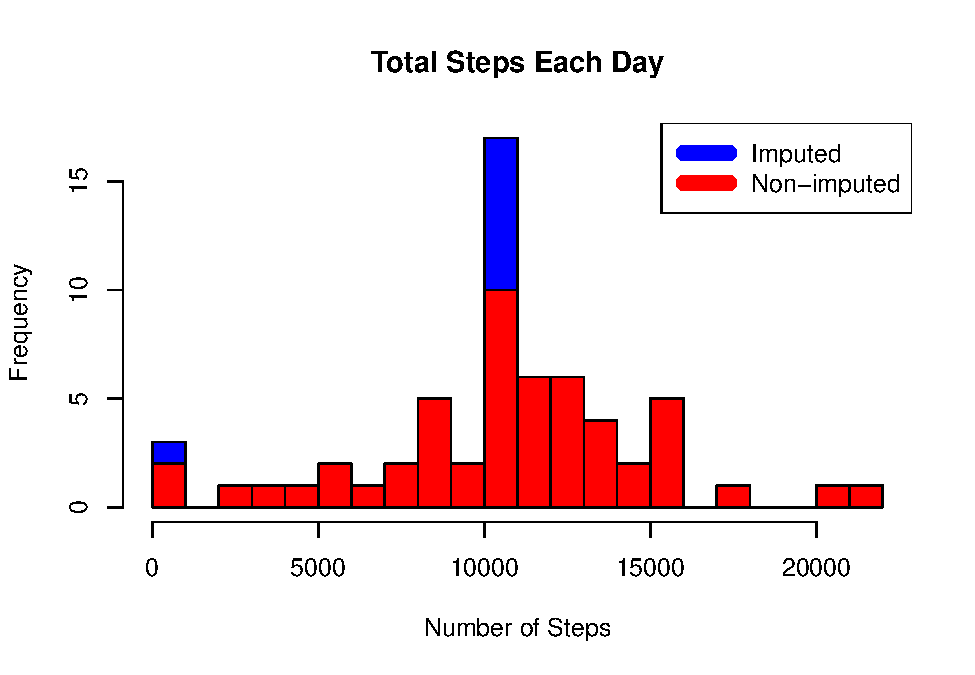
\includegraphics{PA1_template_files/figure-latex/unnamed-chunk-6-1.pdf}

Calculate new mean and median for imputed data.

\begin{Shaded}
\begin{Highlighting}[]
\NormalTok{rmean.i <-}\StringTok{ }\KeywordTok{mean}\NormalTok{(steps_by_day_i}\OperatorTok{$}\NormalTok{steps)}
\NormalTok{rmedian.i <-}\StringTok{ }\KeywordTok{median}\NormalTok{(steps_by_day_i}\OperatorTok{$}\NormalTok{steps)}
\end{Highlighting}
\end{Shaded}

Calculate difference between imputed and non-imputed data.

\begin{Shaded}
\begin{Highlighting}[]
\NormalTok{mean_diff <-}\StringTok{ }\NormalTok{rmean.i }\OperatorTok{-}\StringTok{ }\NormalTok{rmean}
\NormalTok{med_diff <-}\StringTok{ }\NormalTok{rmedian.i }\OperatorTok{-}\StringTok{ }\NormalTok{rmedian}
\end{Highlighting}
\end{Shaded}

Calculate total difference.

\begin{Shaded}
\begin{Highlighting}[]
\NormalTok{total_diff <-}\StringTok{ }\KeywordTok{sum}\NormalTok{(steps_by_day_i}\OperatorTok{$}\NormalTok{steps) }\OperatorTok{-}\StringTok{ }\KeywordTok{sum}\NormalTok{(steps_by_day}\OperatorTok{$}\NormalTok{steps)}
\end{Highlighting}
\end{Shaded}

\begin{itemize}
\tightlist
\item
  The imputed data mean is 10,589.69
\item
  The imputed data median is 10,766.19
\item
  The difference between the non-imputed mean and imputed mean is
  -176.4949
\item
  The difference between the non-imputed mean and imputed mean is
  1.188679
\item
  The difference between total number of steps between imputed and
  non-imputed data is 75363.3. Thus, there were 75,363.32 more steps in
  the imputed data.
\end{itemize}

\subsection{Are there differences in activity patterns between weekdays
and
weekends?}\label{are-there-differences-in-activity-patterns-between-weekdays-and-weekends}

Created a plot to compare and contrast number of steps between the week
and weekend. There is a higher peak earlier on weekdays, and more
overall activity on weekends.

\begin{Shaded}
\begin{Highlighting}[]
\NormalTok{weekdays <-}\StringTok{ }\KeywordTok{c}\NormalTok{(}\DecValTok{2}\NormalTok{, }\DecValTok{3}\NormalTok{, }\DecValTok{4}\NormalTok{, }\DecValTok{5}\NormalTok{, }\DecValTok{6}\NormalTok{); }
\NormalTok{imputed_data}\OperatorTok{$}\NormalTok{dow =}\StringTok{ }\KeywordTok{as.factor}\NormalTok{(}\KeywordTok{ifelse}\NormalTok{(}\KeywordTok{is.element}\NormalTok{(}\KeywordTok{wday}\NormalTok{(}\KeywordTok{as.Date}\NormalTok{(imputed_data}\OperatorTok{$}\NormalTok{date)),weekdays), }\StringTok{"Weekday"}\NormalTok{, }\StringTok{"Weekend"}\NormalTok{))}

\NormalTok{steps_by_interval_i <-}\StringTok{ }\KeywordTok{aggregate}\NormalTok{(steps }\OperatorTok{~}\StringTok{ }\NormalTok{interval }\OperatorTok{+}\StringTok{ }\NormalTok{dow, imputed_data, mean)}

\KeywordTok{library}\NormalTok{(lattice)}

\KeywordTok{xyplot}\NormalTok{(steps_by_interval_i}\OperatorTok{$}\NormalTok{steps }\OperatorTok{~}\StringTok{ }\NormalTok{steps_by_interval_i}\OperatorTok{$}\NormalTok{interval }\OperatorTok{|}\NormalTok{steps_by_interval_i}\OperatorTok{$}\NormalTok{dow, }\DataTypeTok{main=}\StringTok{"Average Steps per Day by Interval"}\NormalTok{,}\DataTypeTok{xlab=}\StringTok{"Interval"}\NormalTok{, }\DataTypeTok{ylab=}\StringTok{"Steps"}\NormalTok{,}\DataTypeTok{layout=}\KeywordTok{c}\NormalTok{(}\DecValTok{1}\NormalTok{,}\DecValTok{2}\NormalTok{), }\DataTypeTok{type=}\StringTok{"l"}\NormalTok{)}
\end{Highlighting}
\end{Shaded}

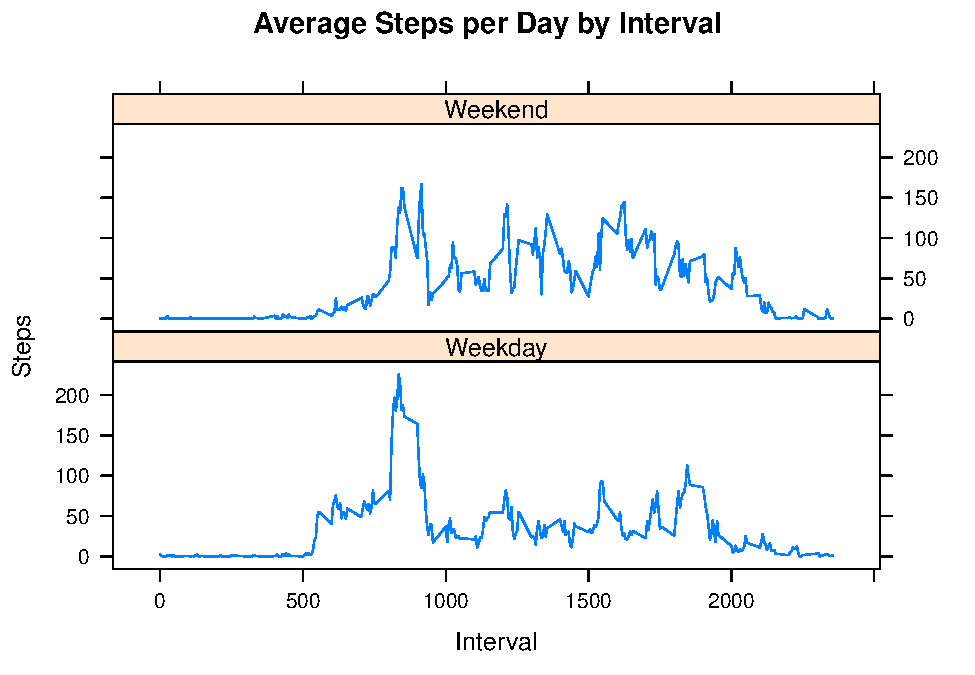
\includegraphics{PA1_template_files/figure-latex/unnamed-chunk-10-1.pdf}


\end{document}
